\documentclass[t]{beamer}

% For more themes, color themes and font themes, see:
% http://deic.uab.es/~iblanes/beamer_gallery/index_by_theme.html
%\usetheme{iclpt}
\usepackage{ragged2e}
\usepackage{etoolbox}
\apptocmd{\frame}{}{\justifying}{}

\apptocmd{\column}{}{\justifying}{}
\hyphenpenalty=1000
\exhyphenpenalty=1000

%
\mode<presentation>
{
  \usetheme{Madrid}       % Madrid or try default, Darmstadt, Warsaw, ...
  \usecolortheme{spruce} % default or try albatross, beaver, crane, beetle, dove, fly, monarca, seagull, spruce, and wolverine ...
  \usefonttheme{serif}    % serif or try default, structurebold, ...
  %\setbeamertemplate{navigation symbols}{}
  \setbeamertemplate{caption}[numbered]
}

\usepackage[english]{babel}
\usepackage[utf8x]{inputenc}
\usepackage{chemfig}
\usepackage[version=3]{mhchem}

\usepackage{enumitem}
\setlist[itemize]{label=\usebeamertemplate{itemize item}}

\usepackage{graphics}
\usepackage{graphicx}
\usepackage{pifont}
\usepackage{amsfonts}
\usepackage{amssymb}
\usepackage{xspace,colortbl}
%\usepackage[screen,panelleft,code,blue,sectionbreak]{pdfscreen}
\usepackage[round]{natbib}
\usepackage{hyperref}
\usepackage{lmodern}
\usetikzlibrary{positioning}
\usepackage[T1]{fontenc}
% On Overleaf, these lines give you sharper preview images.
% You might want to `comment them out before you export, though.
\usepackage{pgfpages}
\pgfpagesuselayout{resize to}[%
  physical paper width=8in, physical paper height=6in]

\newtheorem{thm}{Theorem}[section]
\newtheorem{cor}[thm]{Corollary}
\newtheorem{lem}[thm]{Lemma}
\newtheorem{prop}[thm]{Proposition}
%\theoremstyle{definition}
\newtheorem{defn}[thm]{Definition}
%\theoremstyle{remark}
\newtheorem{rem}[thm]{Remark}
\numberwithin{equation}{section}
% MATH -----------------------------------------------------------
\newcommand{\norm}[1]{\left\Vert#1\right\Vert}
\newcommand{\abs}[1]{\left\vert#1\right\vert}
\newcommand{\set}[1]{\left\{#1\right\}}
\newcommand{\Real}{\mathbb R}
\newcommand{\eps}{\varepsilon}
\newcommand{\To}{\longrightarrow}
\newcommand{\BX}{\mathbf{B}(X)}
\newcommand{\A}{\mathcal{A}}
%\usetheme{iclpt}
\usepackage{url}
\usepackage{amsmath}

%\pgfdeclareimage[height=0.5cm]{university-logo}{eiwr.png}
% \logo{\pgfuseimage{eiwr.png}}
% Here's where the presentation starts, with the info for the title slide

\begin{block}{}
\begin{flushleft}
\begin{figure}
%
\includegraphics[scale=0.35]{images/Fields.pdf}
\end{figure}
\end{flushleft}
\end{block}

\title[Insider Threat]{Insider Threat}
\author[MK, FK, KSS]{Aaron Tronsgard, Kumar Sannidhya Shukla, Brinda Venkataramani}

\date{\today}
\vfill
\begin{document}
\titlepage

% These three lines create an automatically generated table of contents.
\newpage
\begin{frame}{}
\vspace{-6mm}
\small{
 ~~~~~~~~~~~ \tableofcontents
 } \tiny
\end{frame}

\section{Introduction}
\begin{frame}{Introduction}


\justifying{
\begin{itemize}
  \item We were approached by a large tech company for help with their threat alert system. 
\begin{itemize}
\item They have a mature insider threat stack.
\item Includes multiple models, IDS, and threat hunting methods.
\end{itemize}
\pause
\item They receive too many alerts for their security analysts to go through manually, resulting in alert fatigue.
\end{itemize}}

\begin{center}
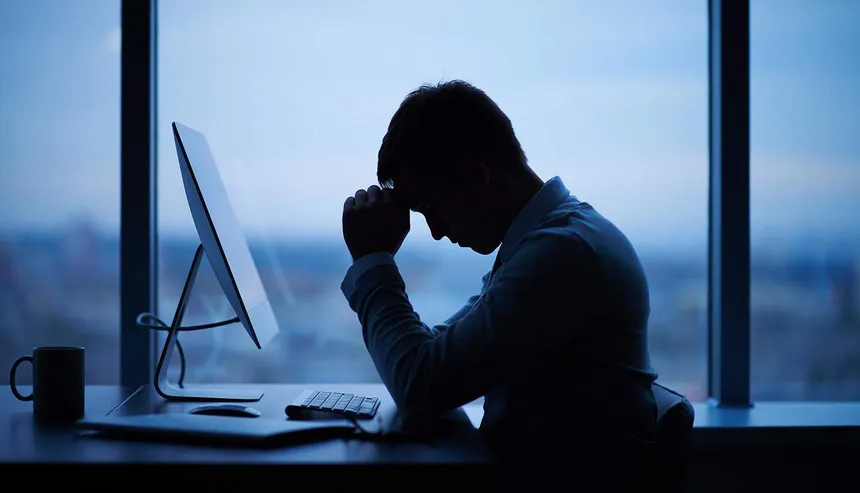
\includegraphics[scale=0.25]{analyst.jpg}
\end{center}
\end{frame}


\begin{frame}{The data}
  \begin{itemize}
    \item What does the data look like? 
    
    \pause 
    
    \item The company's system flags suspicious events and records data about the event and the entities involved.
  \end{itemize}
  
  \pause
  
  \begin{center}
  	Sample Event:
  	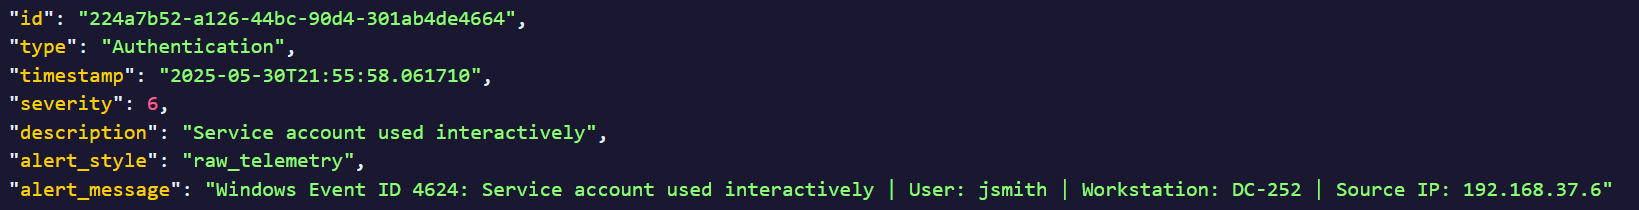
\includegraphics[scale=0.4]{event.png}
  \end{center}
  
  \pause
  
  \begin{center}
  	Sample Entity: \\
  	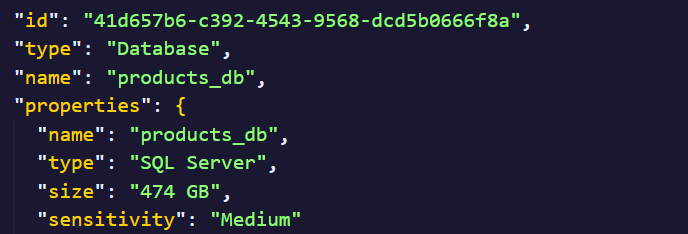
\includegraphics[scale=0.4]{entity.png}
  \end{center}
  
  \pause
  
  \begin{center}
  	Sample Relationship: \\
  	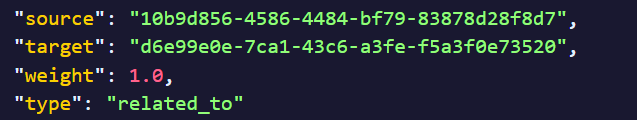
\includegraphics[scale=0.4]{relationship.png}
  \end{center}
\end{frame}

\begin{frame}{Business Needs}
	\begin{itemize}
		\item The data consists of hundreds of events, entities, and relationships between them.
		
		\item This is too much for the analyst to go through every week.
		
		\pause
		
		\item Our goal is to clump events together into potential attack scenarios and provide the analyst with a (much smaller) list of events to look into manually.
	\end{itemize}
	
	\pause
	
	\begin{center}
	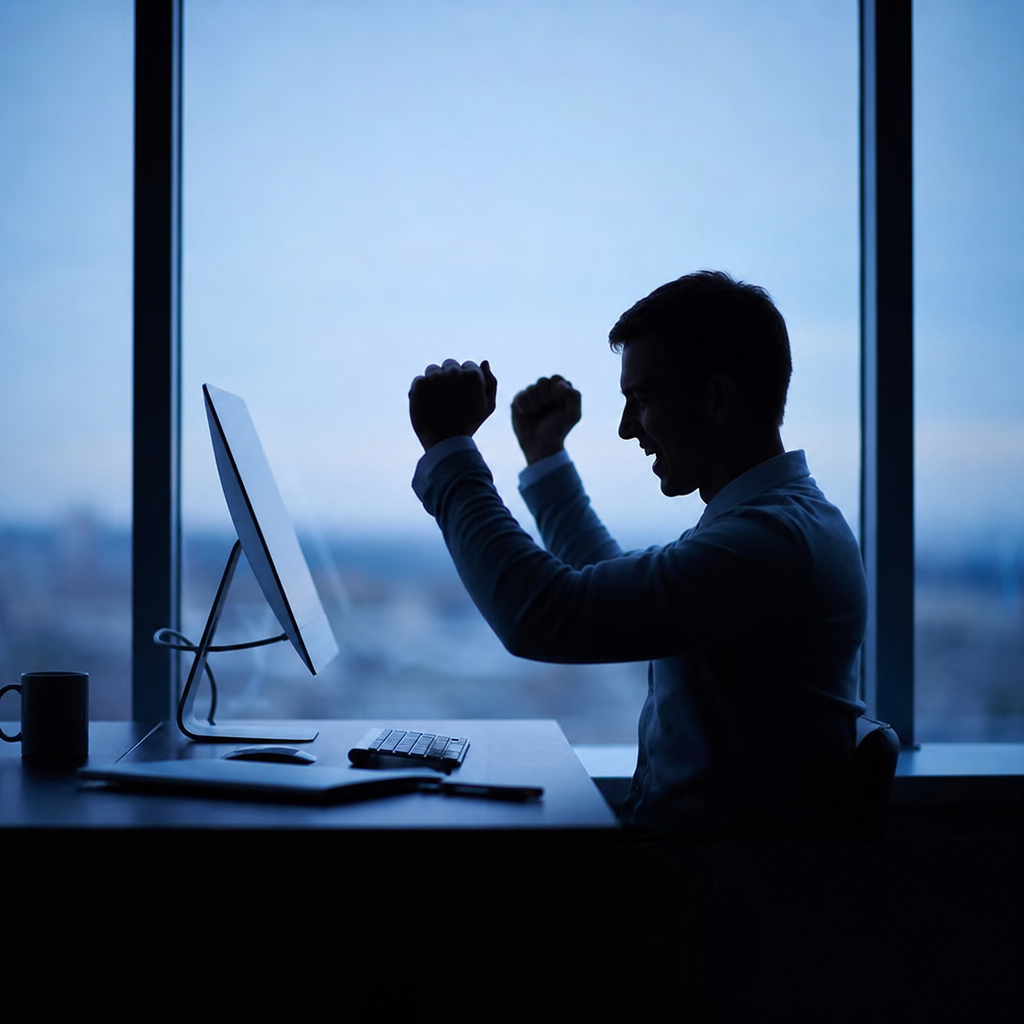
\includegraphics[scale=0.1]{analyst_happy.png}
	\end{center}
\end{frame}

\begin{frame}{Outcomes}
	\begin{itemize}[itemsep = 12 pt, topsep=48 pt]
		\item Success will be measured by our ability to make the analyst's job easier.
		
		\pause
		
		\item Saving the company money and resources, mostly in human-hours, and allowing the analyst to spend more time on other projects.
		
		\pause
		
		\item While also hopefully being able to more reliably alert the company to malicious attack scenarios.
	\end{itemize}
\end{frame}


\section{Methodology (Part 1)}

\begin{frame}{Anomaly detection}
\begin{itemize}
  \item \textbf{Anomaly}: Anomalies are data patterns that have vastly
    different characteristics from \textit{normal} data points.
    \item Anomaly detection provides critical and actionable
      information about the data in various domains:
      \begin{itemize}
        \item Anomaly in credit card transactions $\rightarrow$
          Fraudulent use
        \item Anomaly in astronomical images $\rightarrow$
          New celestial body
        \item Anomaly in network traffic $\rightarrow$
          Potential attack
      \end{itemize}
    \item A naive solution: treat this as a (supervised)
      classification problem
    \item This creates a profile for all \textit{`normal'} data points
      and anomalies are those that do not conform to this profile.
    \begin{itemize}
      \item Slower
      \item Lots of false positive
      \item Susceptible to swamping effect
      \item Feasible only in low dimensions
    \end{itemize}
  \item We will \textbf{Isolation Forests} for anomaly detection.
\end{itemize}
\end{frame}
\newpage

% Slide 2
\begin{frame}{Isolation Forest}
\begin{itemize}
    \item Goal: detect anomalies in high-dimensional data
    \item Key idea: anomalies are ``few and different'',
      whereas, \textit{normal} data points are ``many and similar''.
    \item Instead of modeling normal data, we isolate points
    \item Anomalies are those that isolate \textit{easily}.
\end{itemize}
\end{frame}
\newpage

% Slide 3
\begin{frame}{Core Idea}
\begin{itemize}
    \item Build random binary trees called \textbf{isolation trees}
    \item At each node:
    \begin{itemize}
        \item randomly choose a feature
        \item randomly choose a split value
    \end{itemize}
    \item Anomalies tend to be isolated in fewer splits
    \item Normal points require deeper paths to isolate
\end{itemize}
\end{frame}
\newpage

%\begin{frame}{The Isolation Forest Algorithm}

%\end{frame}

\begin{frame}{Scoring Anomalies}
\begin{itemize}
    \item For each point $x$, compute average path length $h(x)$ over trees
    \item Define anomaly score:
    \[
    s(x, n) = 2^{-\frac{h(x)}{c(n)}}
    \]
    where $c(n)$ is average path length in a binary search tree
    \item High score $\Rightarrow$ more anomalous
\end{itemize}
\end{frame}
\newpage

% Slide 5
\begin{frame}{Algorithm Summary}
\begin{enumerate}
    \item Sample subset of data
    \item Build many isolation trees
    \item Compute path lengths for each point
    \item Aggregate to obtain anomaly score
    \item Flag points with high scores as anomalies
\end{enumerate}

\vspace{0.3cm}
\textbf{Key advantage:} No distance or density estimation required
\end{frame}
\newpage

\begin{frame}{The Data}
\justifying{
\begin{itemize}
  \item The data consist of a single JSON file, consisting
    of 3 arrays \footnote{And perhaps some metadata}:
    \begin{itemize}
      \item \texttt{events} \pause
      \item \texttt{entities} \pause
      \item \texttt{relationships} \pause
    \end{itemize}
  \item \texttt{events} is an array consisting of event objects
    which provide the details about the security incidents like
    timestamp, severity score and description. \pause
  \item \texttt{entities} is an array consisting of entity objects
    which provide the details of the affected entity (which could
    be a user, a host, a file, a process \textit{etc.}.) like
    the type of entity and some metadata about them (like name,
    IP address, department etc.). \pause
  \item \texttt{relationships} array gives us the links between
    events and entities and the \textit{`weight'} of the link. \pause
  \item How do we handle this data?
\end{itemize}}
\end{frame}
\newpage

\begin{frame}{Graphs}
\justifying{
\begin{itemize}
  \item A graph $G$ consist of a pair $(V, E)$ of
    vertices $V$ and edges $E \subseteq {V \choose 2}$.
  \item For example, the following graph
    \begin{center}
    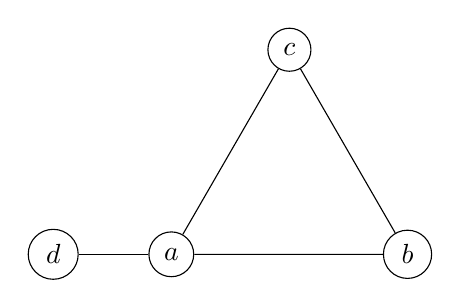
\begin{tikzpicture}[scale=1.5]

    \node[circle,draw] (v1) at (0,0) {$a$};
    \node[circle,draw] (v2) at (2,0) {$b$};
    \node[circle,draw] (v3) at (1,1.732) {$c$};
    \node[circle,draw] (v4) at (-1,0) {$d$};

    \draw (v1) -- (v2) -- (v3) -- (v1);
    \draw (v4) -- (v1);
  \end{tikzpicture}
  \end{center}
  consists of the vertex set $V = \{a, b, c, d\}$
  and the edge set $E = \{\{a, b\}, \{b, c\}, \{c, a\}, \{d, a\}\}$
\end{itemize}}
\end{frame}
\newpage

\begin{frame}{Bipartite Graphs}
\justifying{
\begin{itemize}
  \item  A bipartite graph is a graph whose vertex set $V$
    can be partitioned $G = A \sqcup B$ such that no two vertices
    in $A$ share an edge, and no two vertices in $B$ share an edge.

  \item An example:

    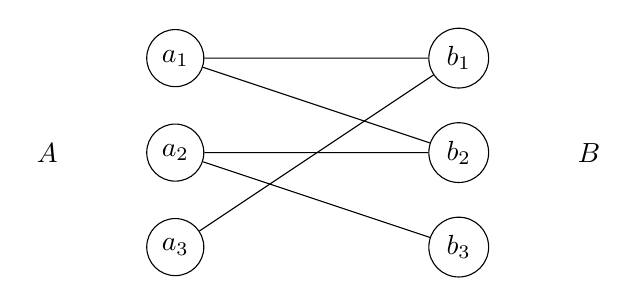
\begin{tikzpicture}[scale=1.2]

% Left part
\node[circle,draw] (u1) at (0,2) {$a_1$};
\node[circle,draw] (u2) at (0,1) {$a_2$};
\node[circle,draw] (u3) at (0,0) {$a_3$};

% Right part
\node[circle,draw] (v1) at (3,2) {$b_1$};
\node[circle,draw] (v2) at (3,1) {$b_2$};
\node[circle,draw] (v3) at (3,0) {$b_3$};

% Labels for the bipartition
\node[left=1cm of u2] {$A$};
\node[right=1cm of v2] {$B$};

% Edges
\draw (u1) -- (v1);
\draw (u1) -- (v2);
\draw (u2) -- (v2);
\draw (u2) -- (v3);
\draw (u3) -- (v1);

\end{tikzpicture} \pause

\item What is a criterion to determine if a graph is bipartite? \pause
\item No odd cycle $\iff$ Bipartite

\end{itemize}}
\end{frame}
\newpage

\begin{frame}{How to handle the data?}
\justifying{
\begin{itemize}
  \item We build a bipartite graph out of the provided data as follows: \pause
  \item We let the vertex set be \texttt{events} $\sqcup$ \texttt{entities}. \pause
  \item We let the edge set be the \texttt{relationships}. \pause
  \item An example:
    \begin{center}
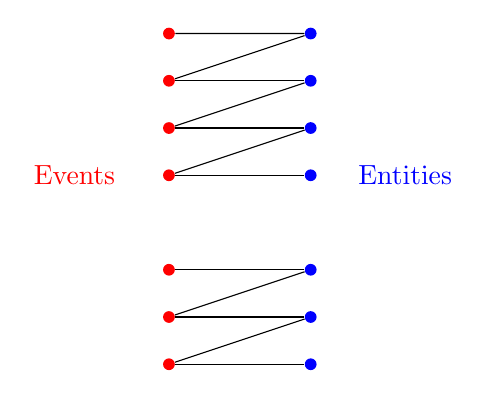
\begin{tikzpicture}[scale=0.6,
    every node/.style={circle,fill,inner sep=1.5pt}]

% Partition labels
\node[draw=none,fill=none, color=red] at (-2,2) {Events};
\node[draw=none,fill=none, color=blue] at (5,2) {Entities};

%========================
% Component 1 (4+4)
%========================

% A-side
\node[color=red] (a1) at (0,5) {};
\node[color=red] (a2) at (0,4) {};
\node[color=red] (a3) at (0,3) {};
\node[color=red] (a4) at (0,2) {};

% B-side
\node[color=blue] (b1) at (3,5) {};
\node[color=blue] (b2) at (3,4) {};
\node[color=blue] (b3) at (3,3) {};
\node[color=blue] (b4) at (3,2) {};

% Edges
\draw (a1)--(b1);
\draw (a2)--(b1);
\draw (a2)--(b2);
\draw (a3)--(b2);
\draw (a3)--(b3);
\draw (a4)--(b3);
\draw (a4)--(b4);

%========================
% Component 2 (3+3)
%========================

% A-side
\node[color=red] (c1) at (0,0) {};
\node[color=red] (c2) at (0,-1) {};
\node[color=red] (c3) at (0,-2) {};

% B-side
\node[color=blue] (d1) at (3,0) {};
\node[color=blue] (d2) at (3,-1) {};
\node[color=blue] (d3) at (3,-2) {};

% Edges
\draw (c1)--(d1);
\draw (c2)--(d1);
\draw (c2)--(d2);
\draw (c3)--(d2);
\draw (c3)--(d3);

\end{tikzpicture}
\end{center}
\pause
\item Observe that this example has 2 connected components.
\end{itemize}}
\end{frame}
\newpage

\begin{frame}{Isolating the anomalous components}
  \justifying{
  \begin{itemize}
    \item We feed the connected components of this graph
      to the isolation forest algorithm.
    \item The pipeline: \begin{center}
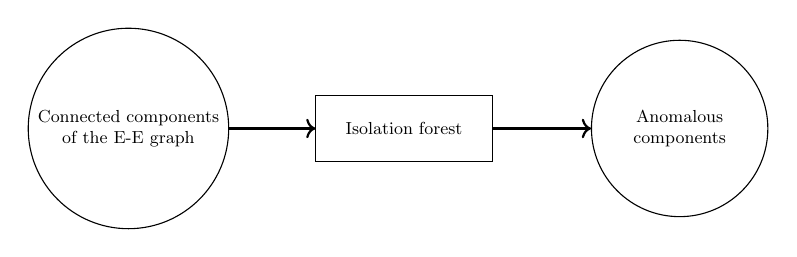
\begin{tikzpicture}[
    scale=0.7,
    transform shape,
    node distance=5cm,
    every node/.style={font=\small},
    circ/.style={circle,draw,minimum width=3.2cm,align=center},
    box/.style={rectangle,draw,minimum width=3.2cm,minimum height=1.2cm,align=center}
]

\node[circ] (start) {Connected components\\of the E-E graph};

\node[box,right of=start] (iso) {Isolation forest};

\node[circ,right of=iso] (end) {Anomalous\\components};

\draw[->,thick] (start) -- (iso);
\draw[->,thick] (iso) -- (end);

\end{tikzpicture}


      \end{center}
    \item The components with high anomaly score are likely
      to be attack scenarios.
  \end{itemize}}
\end{frame}
\newpage

\begin{frame}
  \begin{itemize}
    \item In practice, most hash functions use some kind of
      mixing algorithm that transforms string of length
      $n$ into another string of length $n$.
    \item The hash function breaks the string into blocks
      of length $n$.
    \item $m = m_1 || m_2 || \dots || m_k$.
    \item Then it combines iteratively combines each block
      with the previously computed hash value using the
      mixing algorithm.
  \end{itemize}
\end{frame}


\section{Methodology (Part 2) and Conclusion}

\begin{frame}{Scoring and triage tiers}
\justifying{
\begin{itemize}
  \item Each subgraph is reduced to a fixed feature vector: mean edge
    weight, mean and maximum severity, kill-chain stage coverage, a
    \textit{temporal-order} score, span, and size.
  \item The temporal-order score is the fraction of consecutive
    (time-sorted) events whose MITRE ATT\&CK stage is non-decreasing.
    A genuine attack progresses in order --- Initial Access $\to$
    Privilege Escalation $\to$ Defense Evasion $\to$ Collection $\to$
    Exfiltration --- so it scores $1.0$, whereas uncorrelated noise does not.
  \item An \textbf{Isolation Forest} scores every subgraph without using any
    labels. Its contamination parameter is set from the dataset's
    FP:TP ratio metadata, so the method ports directly to new input files.
  \item Subgraphs are then split into three tiers:
  \begin{itemize}
    \item \textbf{Critical} --- flagged by the model; the analyst must review.
    \item \textbf{Elevated} --- the next $5\%$ by score; review as capacity allows.
    \item \textbf{Low} --- logged, surfaced only on demand.
  \end{itemize}
\end{itemize}}
\end{frame}
\newpage

\begin{frame}{Key performance indicators}
\justifying{
\begin{itemize}
  \item On the provided dataset, the pipeline ingests \textbf{1{,}012} raw
    alerts and decomposes them into \textbf{185} candidate subgraphs.
  \item Only \textbf{8} subgraphs (\textbf{43} events) reach the Critical
    tier --- a \textbf{95.8\%} reduction in the events an analyst must
    triage.
  \item All \textbf{6} ground-truth attack scenarios land in the Critical
    tier: \textbf{100\% recall} at \textbf{75\% precision}. The two
    false positives that accompany them are cheap --- a few minutes of
    review each --- whereas a missed attack is an incident.
  \item Widening to Critical $+$ Elevated still cuts the workload by
    \textbf{90.8\%} while providing a second, lower-priority queue.
\end{itemize}}
\end{frame}
\newpage

\begin{frame}{Performance across datasets}
\justifying{
\begin{itemize}
  \item We ran the identical pipeline on the provided dataset and on two
    independently generated synthetic datasets (same schema, harder
    separation) that carry ground-truth labels.
\end{itemize}
\vspace{0.4em}
\begin{center}
\renewcommand{\arraystretch}{1.3}
\begin{tabular}{lcccc}
\hline
\textbf{Dataset} & \textbf{Events} & \textbf{Subgraphs}
  & \textbf{Recall} & \textbf{Precision} \\
\hline
Provided        & 1{,}012 & 185 & 100\% (6/6) & 75\% \\
Synthetic 1     & 998     & 179 & 83\% (5/6)  & 62\% \\
Synthetic 2     & 997     & 179 & 100\% (6/6) & 75\% \\
\hline
\end{tabular}
\end{center}
\vspace{0.4em}
\begin{itemize}
  \item Recall is measured at the Critical tier. In \textbf{every} dataset,
    \textbf{all 6} attacks fall within Critical $+$ Elevated --- so no
    attack is ever pushed off the analyst's queue.
  \item The single Critical-tier miss (Synthetic 1) is a hard false
    positive that mimics a full kill chain; it still surfaces one tier down.
\end{itemize}}
\end{frame}
\newpage

\begin{frame}{Validating without labels}
\justifying{
\begin{itemize}
  \item Most datasets ship \textbf{no ground-truth labels} --- as in a real
    deployment, where the analyst is the one assigning them. We can still
    sanity-check the output two ways.
  \item \textbf{Against metadata.} The provided unlabeled set declares
    \textbf{3} expected attack scenarios in its metadata. With no access to
    labels, the pipeline flags \textbf{exactly 3} Critical subgraphs ---
    the correct count falls straight out of the FP:TP-driven threshold.
  \item \textbf{Against structure.} The flagged subgraphs share an
    unmistakable profile that noise does not:
\end{itemize}
\vspace{0.3em}
\begin{center}
\renewcommand{\arraystretch}{1.3}
\begin{tabular}{lcc}
\hline
 & \textbf{Critical} & \textbf{Low} \\
\hline
Avg.\ MITRE stages covered & 5.0 / 5 & 2.1 / 5 \\
Avg.\ edge weight          & 1.00    & 0.59 \\
Avg.\ severity             & 7.6     & 2.5 \\
\hline
\end{tabular}
\end{center}
\vspace{0.3em}
\begin{itemize}
  \item Every flagged subgraph spans the \textbf{full kill chain} with
    \textbf{maximal-confidence} edges --- exactly what a true positive
    should look like.
\end{itemize}}
\end{frame}
\newpage

\begin{frame}{Making it legible: subgraph visualization}
\justifying{
\begin{itemize}
  \item \texttt{visualize\_graphs.py} renders each subgraph as a
    \textbf{bipartite graph}: event nodes (coloured by MITRE stage) on one
    side, the users, hosts, files, and domains they touch on the other.
  \item Edge thickness encodes the relationship \textbf{weight}, so a
    high-confidence attack subgraph is visibly denser and more strongly
    connected than a noise cluster --- the analyst sees \textit{why} it
    scored highly at a glance, with no need to read the raw JSON.
  \item The same tool plots the kill-chain timeline and the
    feature distributions, giving a fast, visual second opinion alongside
    the numeric score for any subgraph the analyst wants to inspect.
\end{itemize}}
\end{frame}
\newpage

\begin{frame}{Ranking, not just flagging}
\justifying{
\begin{itemize}
  \item The tier threshold is a convenience, not a gate. Every subgraph
    receives a continuous anomaly score, and the system prints the
    \textbf{top-10 most anomalous} subgraphs regardless of tier.
  \item This matters because the threshold is deliberately conservative.
    An analyst scanning the ranked list can always look one or two places
    \textit{past} the cut-off and investigate anything that stands out to
    them --- a subgraph does not have to be formally flagged to be reviewed.
  \item Nothing is ever hidden: ``Low'' simply means low-priority, not
    discarded. The full ranked list, with the score explanation for each
    subgraph, remains available.
  \item In practice the genuine attacks occupy the very top of the ranking
    (ranks 1--6 on the provided data), so a human reading top-down reaches
    every real incident before any noise.
\end{itemize}}
\end{frame}
\newpage

\begin{frame}{Manpower and cost saved (per batch)}
\justifying{
\begin{itemize}
  \item Industry estimates put average alert triage at roughly
    \textbf{7 minutes} per alert and a fully-loaded SOC analyst at about
    \textbf{\$67/hour} ($\sim$\$48/hr U.S.\ base $\times\,1.4$ for
    benefits and overhead).\footnotemark
  \item Manually triaging all \textbf{1{,}012} alerts $\approx$
    \textbf{118 analyst-hours} $\approx$ \textbf{\$7{,}900} per weekly batch.
  \item Reviewing only the \textbf{43} Critical-tier events takes
    \textbf{$\sim$5 hours} ($\sim$\$340) --- a saving of
    \textbf{$\sim$113 hours} and \textbf{$\sim$\$7{,}600} per week.
\end{itemize}
\vspace{0.4em}
\begin{center}
\renewcommand{\arraystretch}{1.3}
\begin{tabular}{lccc}
\hline
\textbf{Approach} & \textbf{Alerts} & \textbf{Hours} & \textbf{Loaded cost} \\
\hline
Manual (everything)   & 1{,}012 & 118 & \$7{,}900 \\
Critical only         & 43      & 5   & \$340 \\
Critical $+$ Elevated & 93      & 11  & \$730 \\
\hline
\end{tabular}
\end{center}
\footnotetext{Triage time: Prophet Security, \textit{SOC Capacity Modeling}
(2025). Salary: Glassdoor / Salary.com (2026).}}
\end{frame}
\newpage

\begin{frame}{Manpower and cost saved (annualized)}
\justifying{
\begin{itemize}
  \item The provided dataset covers roughly \textbf{one week} of alerts.
    Extrapolating the same volume across a year ($\times 52$):
\end{itemize}
\vspace{0.4em}
\begin{center}
\renewcommand{\arraystretch}{1.3}
\begin{tabular}{lcc}
\hline
\textbf{Approach} & \textbf{Analyst-hours/yr} & \textbf{Loaded cost/yr} \\
\hline
Manual (everything) & $\sim$6{,}100 & $\sim$\$413{,}000 \\
Critical only       & $\sim$260     & $\sim$\$18{,}000 \\
\hline
\textbf{Saved}      & $\sim$5{,}900 & $\sim$\$395{,}000 \\
\hline
\end{tabular}
\end{center}
\vspace{0.4em}
\begin{itemize}
  \item That is roughly \textbf{3 full-time analysts} freed from manual
    triage --- redeployable to deeper investigation and threat hunting ---
    while \textbf{every known attack is still caught}.
  \item Figures are a first-order extrapolation from one week and assume a
    constant alert rate; they are intended to convey scale, not a budgeted
    forecast.
\end{itemize}}
\end{frame}
\newpage

\begin{frame}{Future work: analyst feedback and retraining}
\justifying{
\begin{itemize}
  \item The current model is fully \textbf{unsupervised} --- it needs no
    labels, which is what lets it run on any new input file on day one.
  \item A natural extension is a \textbf{feedback loop}. Each subgraph in the
    ranked output could expose a one-click tag --- \texttt{TRUE\_POSITIVE},
    \texttt{FALSE\_POSITIVE}, or \texttt{NEEDS\_INVESTIGATION} --- written to
    a standardized log alongside the subgraph's feature vector.
  \item Because we already compute a feature vector per subgraph, every tag
    becomes a labelled training example essentially for free. Once enough
    accumulate, they support a \textbf{supervised} layer (e.g.\ logistic
    regression or a random forest) that complements the anomaly score and
    learns this organisation's specific notion of a true threat.
  \item Tags would also let the threshold \textbf{self-calibrate}: repeated
    confirmations just below the cut-off can nudge the contamination
    estimate automatically. This was scoped but left as future work.
\end{itemize}}
\end{frame}
\newpage

\begin{frame}{Conclusion}
\justifying{
\begin{itemize}
  \item We turn a flat stream of \textbf{1{,}012} alerts into a ranked,
    tiered queue, cutting the analyst's triage load by roughly \textbf{96\%}
    --- on the order of \textbf{\$0.4M} and \textbf{3 analyst-FTEs} per year
    --- while catching \textbf{every} known attack on the provided data.
  \item MITRE ATT\&CK kill-chain \textbf{temporal logic} is the key signal:
    it distinguishes coordinated attacks from coincidental clusters of
    high-severity noise, and it is what carries performance over to harder,
    unseen data.
  \item The system is unsupervised at its core and ranking-based at the
    surface: nothing is hidden, the full ordered list is always available,
    and analyst feedback offers a clear path to a self-improving model.
\end{itemize}}
\end{frame}

\end{document}
